\documentclass[letterpaper]{l3doc}

\hypersetup{urlcolor = teal, filecolor = violet}
\usepackage[mono = false]{libertine}
\usepackage{pdfpages,hologo,framed}
\hologoFontSetup{general = \sffamily}
\FrameSep = 0pt
\usepackage[fontset = none]{ctex}
\setCJKmainfont[BoldFont = *-Bold]{LXGW WenKai}
\setCJKsansfont[BoldFont = *-Bold]{LXGW WenKai}
\setCJKmonofont[BoldFont = *-Bold]{LXGW WenKai}
\usepackage[os = mac]{menukeys}
\AddToHook{env/function/before}{\vspace*{-.5\baselineskip}}

\title
{
  \bfseries\cls{litetable} 文檔類:多彩嘅課程表
  \footnote{\url{https://github.com/xiamyphys/litetable}}
}
\author
{
  夏明宇 \texttt{<\href{mailto:xiamyphys@gmail.com}{xiamyphys@gmail.com}>}
  \thanks{\href{https://github.com/ljguo1020}{郭李軍}開發咗讀取 \meta{left} -> \meta{right} 型資料結構糢塊同低版本 \hologo{TeX} Live 相容糢塊.}
}
\date{Version 3.1A, \today}

\begin{document}

\maketitle

\section{介紹}

\cls{litetable} 文檔類提供咗個多彩嘅課程表設計,基於 \cls{article} 文檔類,由 \pkg{expl3} 和 \pkg{tikz} 構建. 相容發行版 \hologo{TeX} Live 2021 同更高版本,喺 \hologo{pdfLaTeX} 同 \hologo{XeLaTeX} 編譯器下均可正常運行. 本文檔系 \cls{litetable} 文檔類嘅用户手冊放,手冊放同時有\href{./litetable-en.pdf}{英文}同\href{./litetable-cn.pdf}{官話}版本\footnote{\href{https://qm.qq.com/q/RyssAhG4qy}{QQ Group: 760570712}}.

\section{載入 \cls{litetable} 並建置課程表框架}

同載入其他文檔類一樣,只令寫下

\begin{framed}
  \begin{verbatim}
    \documentclass{litetable}
  \end{verbatim}
\end{framed}

如果用戶需要輸入中文,可自行載入 \pkg{ctex} 宏包並設置字型.

\begin{function}{\timelist,\weeklist}
  \begin{syntax}
    \cs{timelist}\oarg{rows}\marg{time list}             \cs{timelist}\marg{time list}\oarg{rows}
    \cs{weeklist}\oarg{default weeks}\marg{week list}    \cs{weeklist}\marg{week list}\oarg{default weeks}
  \end{syntax}

  以上命令均有兩個參數. 命令 \cs{timelist} 嘅可選參數可直接決定課程表嘅行數,命令 \cs{weeklist} 嘅可選參數可決定預設嘅星期數目並會喺每課程塊嘅嘅右下角顯示. 兩個命令嘅強制參數均接受數組,可分別就系課程表嘅左側添加時間表、喺課程表嘅頂部添加對應寬度比例工作日.
  
  若命令 \cs{timelist} 中時間數組數字大於可選參數接受值,就多餘嘅時間數組將畀忽略,並返回一個警告. 如果只系課程表左側添加一部序號,令強制參數為空即可.
\end{function}

\begin{function}{\more}
  \begin{syntax}
    \cs{more}\marg{comment}
  \end{syntax}

  此命令可喺頁面嘅嘅右下角添加備注.
\end{function}

\begin{function}{\maketable}
  \begin{syntax}
    \cs{maketable}\oarg{semester}\marg{title}            \cs{maketable}\marg{title}\oarg{semester}
  \end{syntax}

  此命令有兩個參數,可建置一個空白嘅課程表框架,使喺命令 \cs{timelist} 同 \cs{weeklist} 後,並喺帶有 \cmd{remember picture,overaly} 選項嘅 \env{tikzpicture} 環境中執行. 可選參數可喺頁面嘅嘅右度角添加學期,強制參數可指定標題.
\end{function}

\section{添加課程塊}

\begin{function}{\course}
  \begin{syntax}
    \cs{course}\oarg{keyvals}\marg{start number}\marg{end number}
  \end{syntax}

  \cs{course} 命令可喺當前工作日添加課程塊,要喺命令 \cs{maketable} 後,並喺帶有 \cmd{remember picture,overaly} 選項嘅 \env{tikzpicture} 環境中執行.
  
  此命令有三個參數. 第一個可選參數接受下列鍵:\keys{\cmdmac~color} \keys{\cmdmac~subject} \keys{\cmdmac~location} \keys{\cmdmac~teacher} \keys{\cmdmac~weeks}. 鍵 \keys{\cmdmac~color} 默認值為 \cmd{teal},鍵 \keys{\cmdmac~weeks} 默認值由命令 \cs{weeklist} 嘅可選參數決定. 第二個同第三個強制參數勒分別為課程嘅開始同結束序號.
  
  \cs{course} 命令嘅用例如下:將此課程塊嘅顏色設置為 \cmd{DarkSlateGray},此課程名為 \cmd{litetable},上堂地方為 \cmd{Hong Kong},老師為 \cmd{M.Y. Xia},喺當日嘅第 \cmd{8} 節課開始,第 \cmd{8} 節課結束.

  \begin{framed}
    \begin{verbatim}
      \course [ color = DarkSlateGray, subject = litetable,
                location = Hong Kong, teacher = M.Y. Xia
              ] {8} {8}
    \end{verbatim}
  \end{framed}

\begin{itemize}[topsep = 0pt]
  \item 若課程塊高度得一格,即$\marg{start number} = \marg{end number}$,就鍵 \keys{\cmdmac~location} 同 \keys{\cmdmac~teacher} 嘅值將輸出喺同一行並以逗號 (,) 隔,鍵 \keys{\cmdmac~weeks} 嘅值將會隱藏.
  \item 若鍵 \keys{\cmdmac~location} 同 \keys{\cmdmac~teacher} 均未賦值,就鍵 \keys{\cmdmac~subject} 嘅值將輸出喺課程塊中心.
  \item 超出課程表工作日範圍嘅課程塊將唔會顯示,只會返回一條警告.
\end{itemize}
\end{function}

\begin{function}{\newday}
  \begin{syntax}
    \cs{newday}\oarg{integral value}
  \end{syntax}

  此命令有一個可選參數,可令其後面添加嘅課程塊後移 \meta{intergal value} 個工作日. 可選參數嘅默認值為\cmd{1},即後移\cmd{1}個工作日.
\end{function}

\clearpage

\section{最小工作範例}

此MWE建置嘅课程表有13行但系得前12行标注时间,课程表顶部共有五个工作日,工作日之间嘅宽度比例为$4:5:4:6:5$,键 \keys{\cmdmac~weeks} 嘅默认值畀赋为 \cmd{Weeks 1 - 16}. 添加咗註解同兩個課程塊.

\begin{framed}
  \begin{verbatim}
    \documentclass{litetable}

    \begin{document}

    \timelist[13]
    {
      08:05 -> 08:50, 08:55 -> 09:40, 10:00 -> 10:45, 10:50 -> 11:35,
      11:40 -> 12:25, 13:30 -> 14:15, 14:20 -> 15:05, 15:15 -> 16:00,
      16:05 -> 16:50, 18:30 -> 19:15, 19:20 -> 20:05, 20:10 -> 20:55
    }
    \weeklist[Weeks 1 - 16]
    {
      Mon -> 4, Tue -> 5, Wed -> 4, Thu -> 6, Fri -> 5
    }
    \more{Author: Mingyu Xia \& Lijun Guo}

    \begin{tikzpicture}[remember picture, overlay]
      \maketable
      \course [ subject = Keep on {\TeX}ing
              ] {10} {11}
      \newday
      \course [ color = DarkSlateGray, subject = litetable,
              location = Hong Kong, teacher = M.Y. Xia
              ] {8} {8}
    \end{tikzpicture}

    \end{document}
  \end{verbatim}
\end{framed}

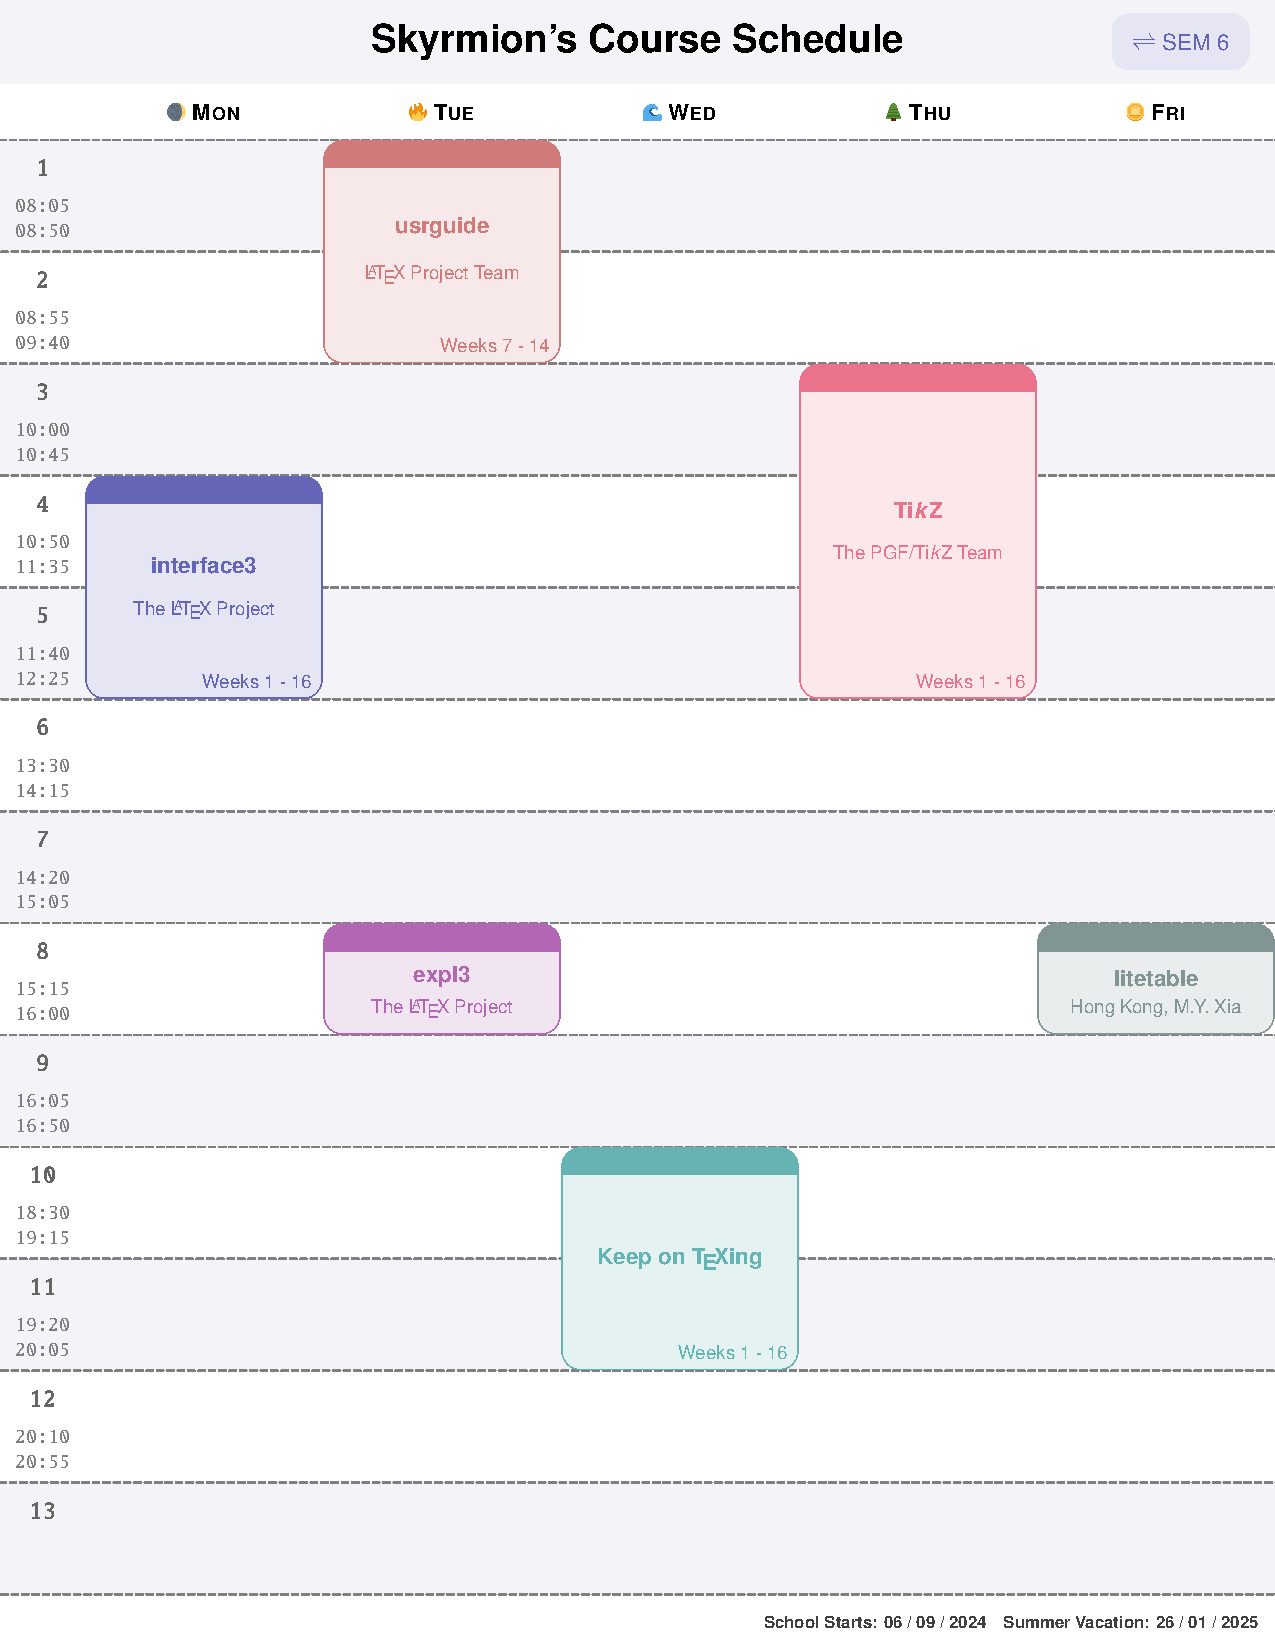
\includepdf[pages = 1]{litetable-demo.pdf}

\end{document}